\subsection{Clustering} \label{sec:clustering}

% \begin{figure}
%     \centering
%     \subfloat[raw data]{
%     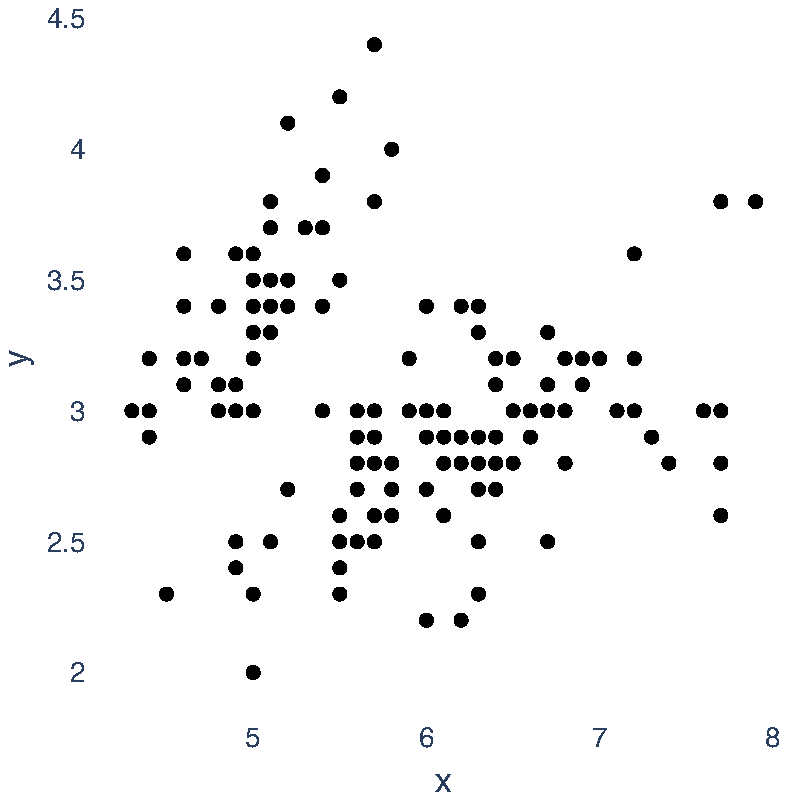
\includegraphics[width=0.5\textwidth]{figures/410_method/kmeans/kmeans_data.pdf}
%     }
%     \subfloat[initialization]{
%     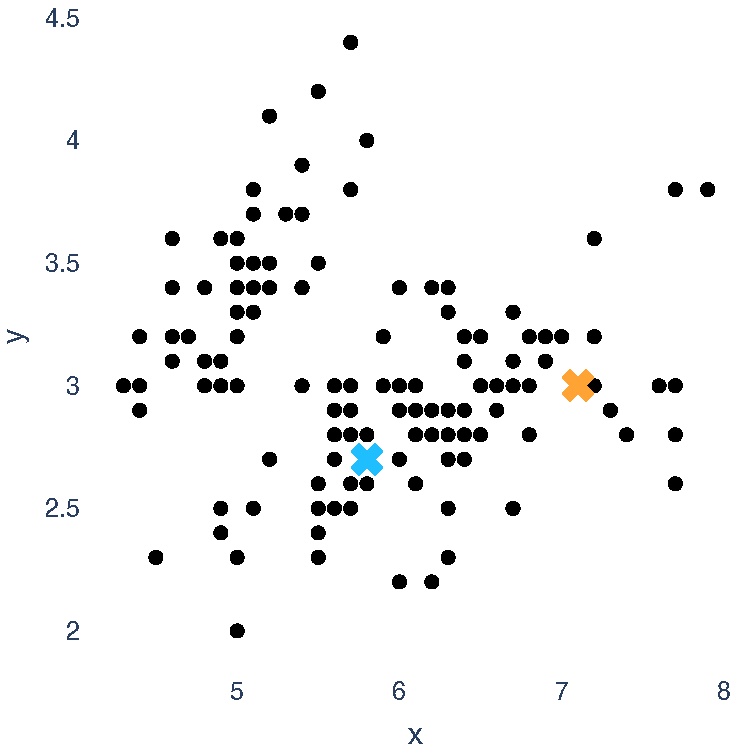
\includegraphics[width=0.5\textwidth]{figures/410_method/kmeans/kmeans_centroid2.pdf}
%     }
    
%     \subfloat[update clusters]{
%     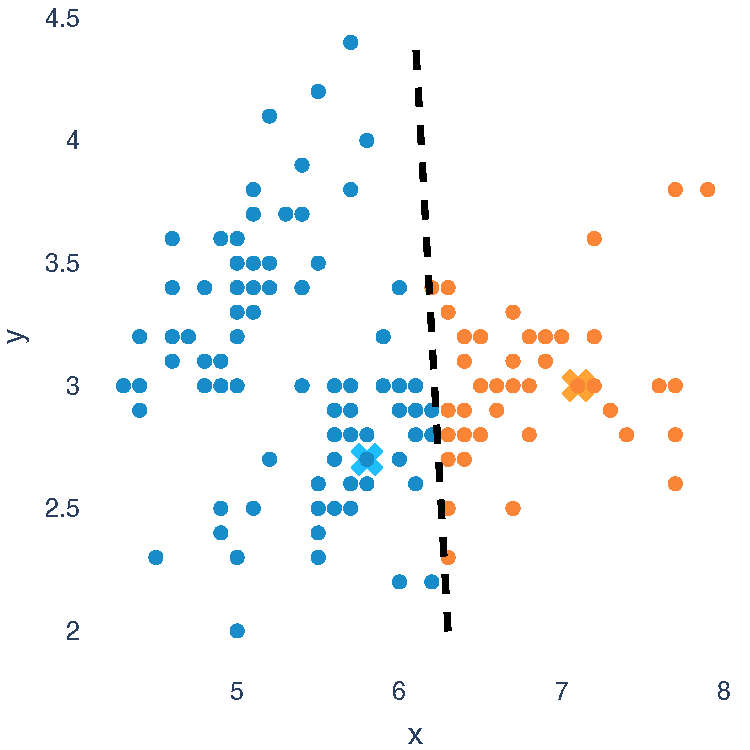
\includegraphics[width=0.5\textwidth]{figures/410_method/kmeans/kmeans_updateCluster.pdf}
%     }
%     \subfloat[update centroids]{
%     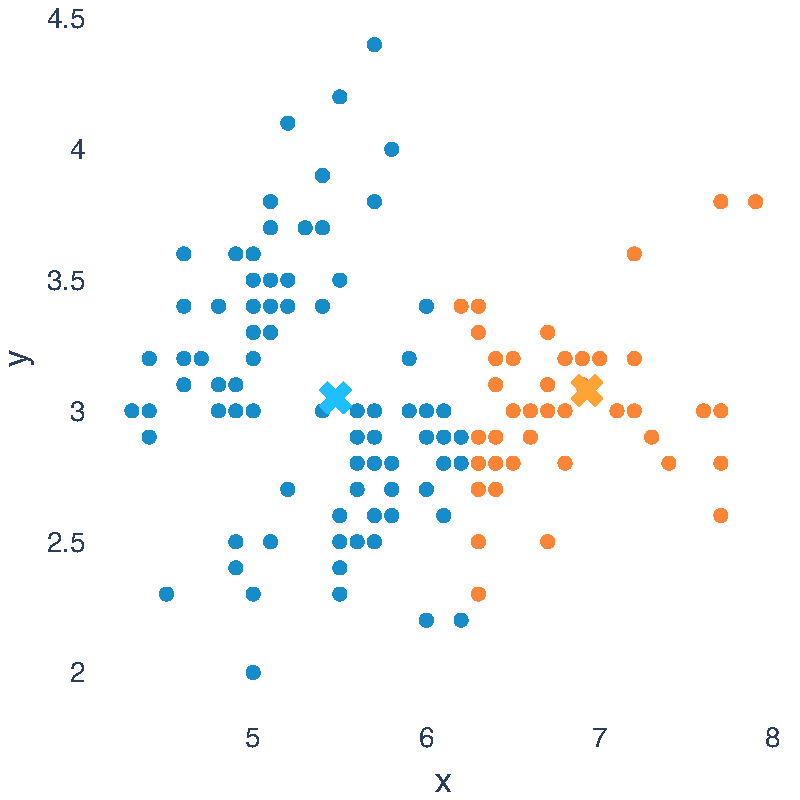
\includegraphics[width=0.5\textwidth]{figures/410_method/kmeans/kmeans_updateCentroids.pdf}
%     }
%     \caption{\textbf{K-Means clustering.} The algorithm performs an iterative search by alternately grouping observations around cluster centers of mass and updating such centroids.}
%     \label{fig:kmeans-pipeline}
% \end{figure}

% \documentclass[]{standalone}
% \usepackage{graphicx,animate} % for \animategraphics
% \begin{document} %http://mirrors.ctan.org/macros/latex/contrib/animate/animate.pdf

\begin{figure}
    \centering
    \animategraphics[width=\textwidth, %loop,
    autoplay]{1}{./figures/410_method/kmeans/gif1/kmeans_}{0}{6}
     \caption{\textbf{K-Means clustering.} The algorithm performs an iterative search by alternately grouping observations around cluster centers of mass and updating such centroids.}
    \label{fig:kmeans-pipeline}
\end{figure}

    
% \begin{figure}
%     \centering
%     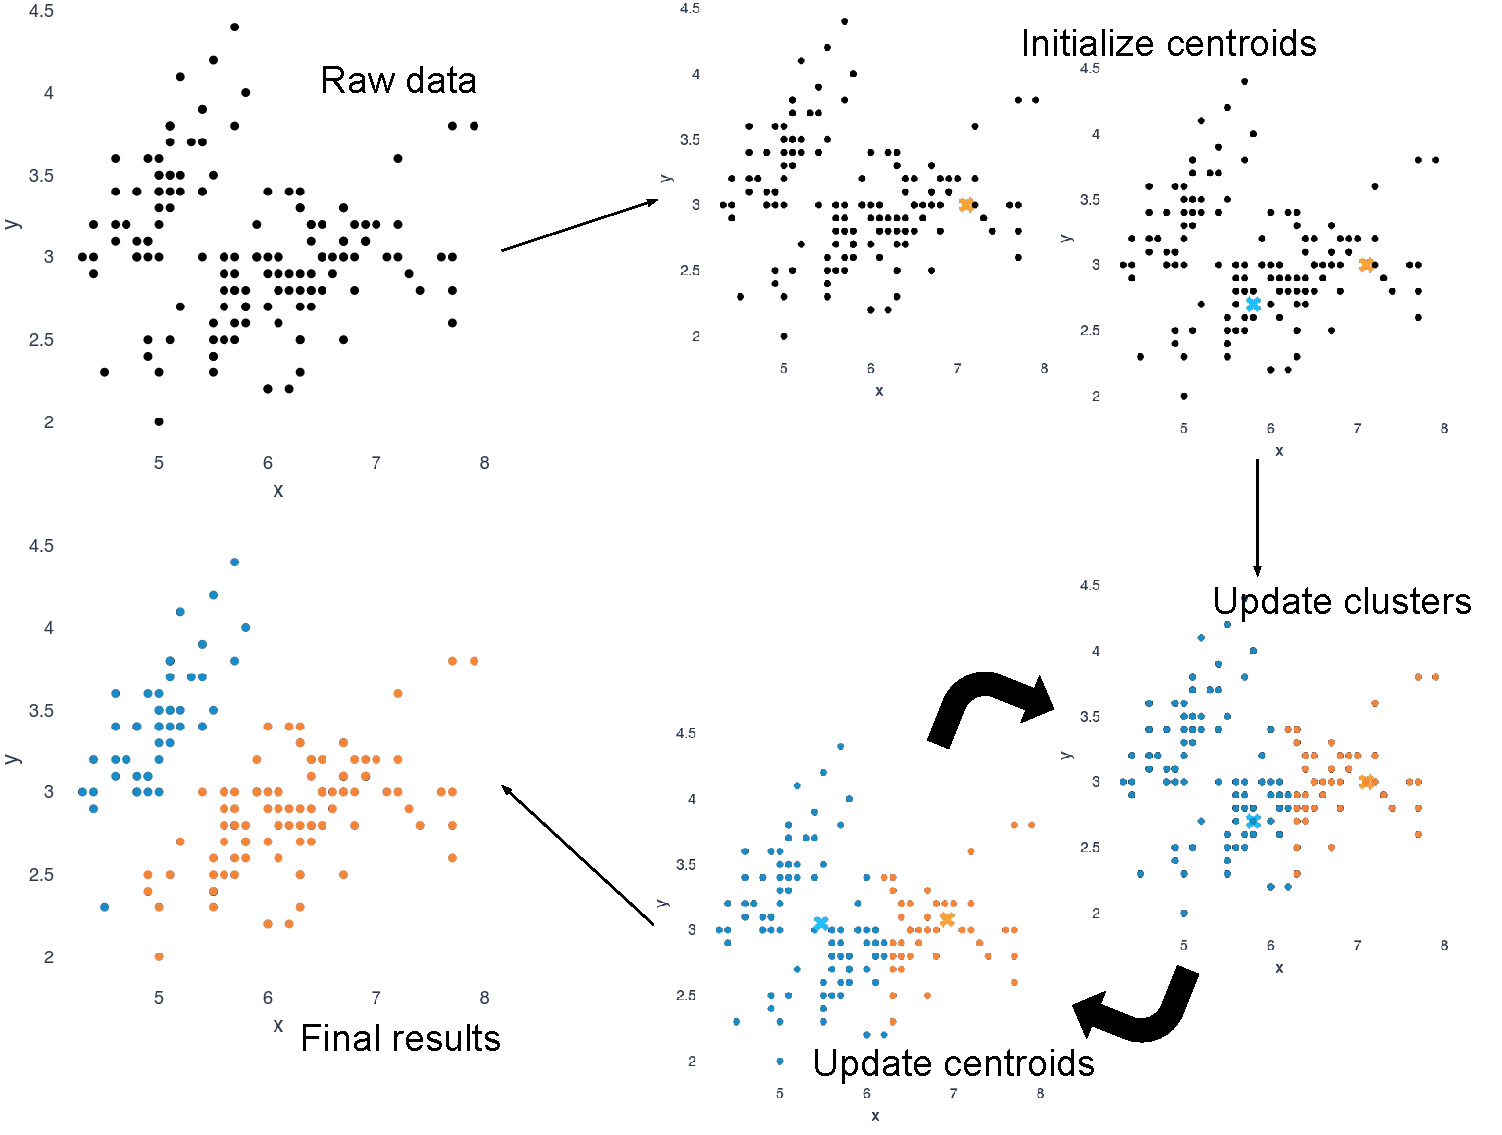
\includegraphics[width=\textwidth]{figures/410_method/kmeans/K-Means++ diagram.pdf}
%     \caption{\textbf{K-Means clustering.} The algorithm performs an iterative search by alternately grouping observations around cluster centers of mass and updating such centroids.}
%     \label{fig:kmeans-pipeline}
% \end{figure}

The next step of the pipeline is the clustering stage.
Cluster analysis examines the task of grouping a set of objects based on a given measure of distance or similarity.
This is a well-studied task typically conducted to discover underlying structures in data during exploratory analysis or pattern recognition.

One of the most intuitive and widely adopted strategies to tackle this problem is the so-called \textit{k-means} algorithm \cite{lloyd1982kmeans}.
This technique is an iterative local search solution, and it refers to a particular formulation of the problem where the number of output groups, $k$, is supposedly known.
The algorithm evolves in four simple steps, starting from this prior information and after establishing a suitable distance measure to express the similarity between data points.
In the initialization phase, $k$ arbitrary centers (also named \textit{centroids}) are chosen uniformly at random from the data points. 
In the next step, the data are split into clusters by mapping each data point to the nearest center. 
Once the groups are formed, the centroids are re-computed as the center of mass of all points assigned to the corresponding cluster.
Finally, the last two steps are repeated until a convergence criterion is met.
\Cref{fig:kmeans-pipeline} illustrates an animation of the first iteration and the final result of the algorithm described above applied to some toy data points.
 
In this study, we resort to clustering for grouping messages which include similar content.
The resulting clusters are therefore interpreted as error categories.
In particular, we adopt a slight variation of the above algorithm referred to as \textbf{k-means++} \cite{arthur2006kmeans++}.
The two techniques share the same workflow except for how the initial centroids are initialized.  
Specifically, the initial step of k-means assign equal probability to all the data points and then samples $k$ centers.
For k-means++ instead, only the first centroid is chosen uniformly at random, while the following $k-1$ are sampled with probability inversely proportional to their distance to the closest predefined centroid.
This careful seeding strategy ensures the initial centers are more spread across the data points, thus favoring better clustering results and a faster convergence.

In order to demonstrate the approach, we report the analysis of FTS data from one full day of operation (2021-01-15), corresponding to roughly 1M errors.
To help the successive evaluation phase, only transfers between Tier-0, Tier-1s and Tier-2s are considered in the analysis.
In practice, more hyper-parameter configurations are explored to test the effect of different choices.
The first set of investigations regards the measure of similarity adopted to form the clusters. 
In this respect, we tested two alternatives, cosine similarity and the classical euclidean distance.
The former consistently outperformed euclidean distance in all attempted experiments, both considering clusters compactness and separation and in terms of interpretability of the results. For this reason, only the the analysis involving \textit{consine similarity} is reported in the following.

Another crucial hyper-parameter is given by the assumed number of clusters, $k$. This represents the number of error categories in our case, which is not known in advance. 
Therefore a grid search for $k \in [12, 15, 20, 30] $ is exploited to retrieve a reasonable estimate from the data.
For this purpose, two geometrical criteria are considered to compare results of different settings, namely the Within cluster Sum of Squared Errors (WSSE) and the Average Silhouette Width (ASW) \cite{rousseeuw1987ASW}.
The WSSE is a measure of the clusters internal variability so the lower its value, the better the performance.
In terms of its definition the WSSE is based on the total sum of squared distances between the points of each group and the correspondent centroid:
\begin{equation}
    \text{WSSE}\left(\text{dist}, k\right) = 
    \sum_{j=1}^{k}{ 
    \sum_{x_i \in C_j}{\text{dist}\left( x_i - \bar{x}_j\right)} 
    }
\end{equation}
where $x_i$ is a generic data point, ${dist}$ is a desired distance measured, and $C_j$ and $\bar{x}_j$ indicate a generic cluster and its centroid, respectively.
Although compactness is certainly a desirable property for the output groups, this metric is strongly affected by the scale of the variables and the number of observations. Indeed, the clusters exhibit a greater variability as their points present higher values and/or the cluster size increases, thus causing the WSSE to explode. 
Also, being unbounded by its nature, i.e. $\text{WSSE} \in \left[ 0, +\inf \right]$, the WSSE is of difficult interpretation on its own and it only makes sense when compared to other values. \\
% In fact, its absolute value have little sense on its own, and it only takes meaning when compared to other.
A better metric is the so-called \textit{average silhouette width}. In brief, the ASW is a measure of clustering performance that accounts for both internal homogeneity and external separation of the clusters.
In particular, let $\bar{a}_i$ be the average distance of $x_i$ from all the other points belonging to the same cluster $C_I$. Also, let $b_i$ be the minimum average distance of $x_i$ from the observations in all the other clusters $C_j , \forall j \neq I$. Then, the ASW is defined as:
\begin{equation}
    \text{ASW}\left(\text{dist}, k\right) = 
    \dfrac{1}{n} \sum_{i=1}^{n}{ 
    \dfrac{b_i - \bar{a}_i}{ max\left( \bar{a}_i, b_i \right) }
    }
\end{equation}
where $n$ is the total number of observation, i.e. error messages in our case.
The average silhouette is much more intuitive to use than the WSSE as its value is bounded in the interval $\left[ -1, +1 \right]$, thus making it far more interpretable.
In practice, negative values of the ASW mean that points of one cluster are on average more similar to observations of other groups than the ones of their own cluster. A value of 0, instead, suggest that the groups are not really distinguishable, thus making the assignation of single observations to any of the clusters almost indifferent.
Finally, positive values close to 1 testify that the clustering produces nicely homogeneous groups that are also well separated among each other.
Given the more intuitive reading of ASW values, the latter is used in the following as the main figure of merit.

% Apart from the distance and the value of $k$, the other hyper-parameters were not optimized and the values \textbox{initSteps=200}, \textbox{tol=0.0001}, \textbox{maxIter=100} were chosen.

The results of the comparison between WSSE and ASW for different values of $k$ are reported in \cref{fig:k_optim}.
Both indicators tend to improve as the number of clusters increases.
In particular, a value of $k=30$ clusters seems to be optimal according to both metrics.
Notably, however, the ASW indicator reaches very high values (around 0.9) even for lower $k$ values.
% of 0.9405 which is a very high score for this metric.
For this reason, the configuration having $\boldsymbol{k=15}$ is preferred to limit the number of suggested issues and minimize the shifters effort.
% considered for the discussion in \cref{ch:opint-results}. 

\begin{figure}
    \centering
    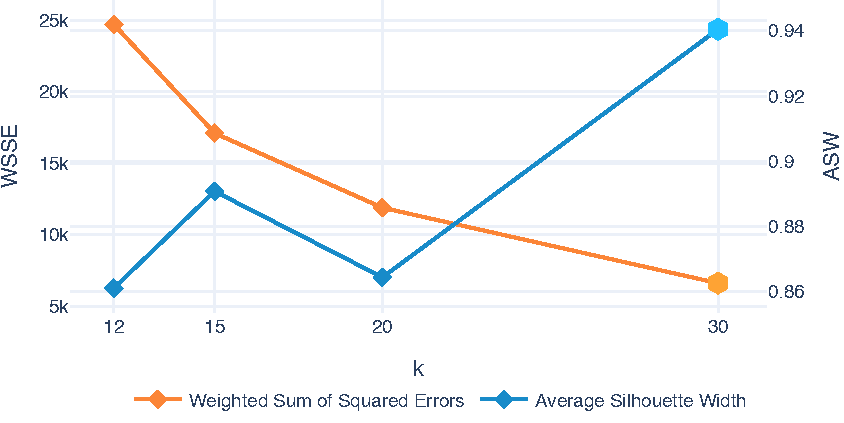
\includegraphics[width=\textwidth]{figures/410_method/kmeans/k_optim.pdf}
    \caption{\textbf{Optimization of $\boldsymbol{k}$.} The plot shows the value of the WSSE and ASW metrics as a function of the number of clusters $k$. The hexagonal markers indicate the optimal values, which correspond to $k=30$ for both indicators.}
    \label{fig:k_optim}
\end{figure}
